
\documentclass[10pt,twocolumn,letterpaper]{article}
\usepackage{cvpr}
\input{preamble}
\definecolor{cvprblue}{rgb}{0.21,0.49,0.74}
\usepackage[pagebackref,breaklinks,colorlinks,allcolors=cvprblue]{hyperref}


\title{SoccerNet Re-Identification Challenge}
\author{
Crea Michelangelo 1993024 \and Gautieri Alessandro 2041850\\
}

\begin{document}
\maketitle

\section*{Abstract}
This report outlines the various phases of the project dedicated to Player Re-Identification (Re-ID) across different matches. First, we explain the project's goal by introducing the \textit{SoccerNet Re-Identification Challenge}: this competition served as our starting point, providing both the necessary datasets and a baseline to benchmark our training.

In the second step, we detail the dataset and how the data was prepared. In this section, we describe the cleaning and \textit{preprocessing} procedures applied to the images to make them suitable for processing by our models.

Next, the document describes the techniques and architectures we selected. We explain how the individual models work and, most importantly, how we combined their predictions into a final \textbf{Ensemble} strategy to achieve better results than using a single model alone.

Following this, we present the concrete results. We report the performance achieved by each individual model and the final ensemble, supported by test values and metrics calculated to measure the system's accuracy.

Finally, we analyze the conclusions drawn from the work and look ahead, proposing potential improvements and future developments to make the project even more effective.


\section{Introduction}
The SoccerNet Re-Identification (ReID) Challenge presents a complex computer vision problem: re-identifying soccer players across multiple camera views in broadcast video footage. This task is complicated by factors such as low resolution, motion blur, occlusion, and similar player appearances (team kits).

Figure~\ref{fig:multiview} illustrates the core challenge: given a player detected in one camera view (query), the system must identify all instances of the same player in other camera views (gallery). The colored lines represent identity associations across views, with different colors indicating different players. This multi-view matching must account for drastic appearance changes due to viewpoint, scale, and occlusion.

\begin{figure}[h]
\centering
\includegraphics[width=\linewidth]{figures/multiview_links.png}
\caption{Multi-view person re-identification in broadcast soccer footage. Players detected in different camera views (top and bottom rows) are linked by identity. Each color represents a different player identity, with lines connecting the same person across views. The challenge involves matching players despite significant variations in pose, scale, and viewpoint.}
\label{fig:multiview}
\end{figure}

To address these challenges and maximize performance, we adopted a multi-model ensemble strategy. Leveraging distinct architectures allows us to capture complementary features, improving the robustness of the re-identification process.

Our approach was also shaped by significant computational constraints. We operated in a heterogeneous hardware environment due to the enormous size of the SoccerNetV3 dataset, training large-scale models on a single consumer-grade machine was infeasible within reasonable timeframes.

\section{Dataset and Preprocessing}
We utilized the SoccerNet-v2 dataset \cite{soccernetv2, soccernetReID}, a large-scale benchmark for holistic understanding of broadcast soccer videos. For the ReID task, the dataset provides bounding box annotations and identity labels across distinct actions and camera angles.

\subsection{Analysis of Input Signal Quality}
The reliability of any biometric system is intrinsically tied to the quality of the input signal ($S_N$) \cite{jain2004introduction}. In contrast to controlled biometric deployments (e.g., fingerprint readers or iris scanners in well-lit environments), sports broadcast footage introduces a complex set of unconstrained degradation factors that make feature extraction significantly more challenging.

We identify the following primary quality degradation sources in the SoccerNet dataset:
\begin{itemize}
    \item \textbf{Motion Blur}: The rapid and often non-linear movement of players, combined with high-speed panning of broadcast cameras, introduces significant temporal blur in individual frames. This smears the spatial frequencies that carry distinctive appearance information (e.g., jersey numbers, distinguishing logos).
    \item \textbf{Resolution Variability}: Player crop resolution varies dramatically depending on broadcast zoom level and the player's distance from the camera. At low resolutions, fine-grained details are entirely lost, leaving only coarse color and shape information.
    \item \textbf{Viewpoint and Pose Variation}: The multi-camera nature of soccer broadcasts implies the same player can be captured simultaneously from drastically different viewpoints and at different body poses, generating large within-class appearance variance.
    \item \textbf{Occlusion}: Players frequently occlude each other during play, resulting in partial observations during detection.
    \item \textbf{Illumination Changes}: Matches take place under diverse lighting conditions across different stadiums, time of day, and weather, causing significant color and contrast shifts across samples.
\end{itemize}

These factors collectively reduce the \textbf{signal-to-noise ratio (SNR)} of the biometric input. From a biometric systems perspective, a degraded input signal is more likely to lead to a degraded biometric template, which in turn increases both the False Rejection Rate (FRR) and the False Acceptance Rate (FAR) of the system. This motivates the selection of models that are explicitly designed to be robust against such variability. Preprocessing steps such as random erasing and color jitter applied during training can be interpreted as \textit{quality-aware data augmentation}, simulating the real-world degraded conditions the model will encounter at test time.

Given the challenge's scale and these signal degradation factors, effective preprocessing was crucial. We adhered to standard ReID practices, including resizing images to a fixed resolution and applying data augmentation techniques such as random erasing, flipping, and color jittering to prevent overfitting and improve robustness against poor signal quality.

\section{Methodology}

\subsection{Biometric System Architecture}

While person re-identification is fundamentally a computer vision task, it maps precisely onto the architecture of a biometric recognition system \cite{jain2004introduction}. Understanding this mapping is crucial to interpret our evaluation methodology.

\textbf{Processing Pipeline.} Our system follows the standard biometric data flow. Each input image (query or gallery) passes through a \textbf{feature extraction} module (one of our trained deep learning models) that outputs a compact, fixed-dimensional \textbf{biometric template}, i.e., the feature vector. At matching time, a \textbf{comparator} computes the \textbf{Squared Euclidean Distance} between the probe template $q$ and every gallery template $g_j$. Specifically, we compute a \textbf{Distance Matrix} $D \in \mathbb{R}^{M \times N}$ (where $M$ is the number of queries and $N$ the number of gallery images), where each entry $D_{i,j} = \|q_i - g_j\|_2^2$ represents the dissimilarity between query $i$ and gallery candidate $j$. The resulting ranked list of gallery candidates, sorted by increasing distance, is then used to measure system performance.

\textbf{Operational Mode: 1:N Open-Set Identification.} Our system operates in the most challenging biometric mode: \textbf{1:N Open-Set Identification}. The key characteristics are:
\begin{itemize}
    \item \textbf{1:N}: Given a probe (one query player), the system must be ranked against an entire gallery of $N$ identities, rather than a single claimed identity (1:1 Verification).
    \item \textbf{Open-Set}: Unlike Closed-Set identification (which assumes the probe identity is always in the gallery), the Open-Set scenario requires the system to also handle rejection. A probe whose closest gallery distance exceeds a decision threshold $\tau$ should be classified as \textit{unknown}, modeling the real case where referees, staff, and players from other matches may appear in the probe set but are absent from the gallery.
\end{itemize}

\textbf{Decision Threshold.} In a production deployment, the threshold $\tau$ establishes a fundamental trade-off: lowering $\tau$ reduces False Acceptances (wrongly claiming a match) but increases False Rejections (failing to identify a genuine match). This trade-off is fully characterized by the Detection Error Trade-off (DET) curve and quantified by the Equal Error Rate (EER), both discussed in Section~\ref{sec:biometric_eval}.

Our core methodology centers on an ensemble of three distinct deep learning models to act as robust feature extractors. By combining the strengths of different architectures, we aim to achieve a higher mean Average Precision (mAP) and Rank-1 accuracy than any single model could achieve in isolation. The idea is that different models learn different feature representations; fusing them can smooth out individual prediction errors.

The three models selection was driven by the need for diversity:
\begin{enumerate}
    \item \textbf{DINOv2}: A Vision Transformer (ViT) based on self-supervised learning, excellent for capturing semantic context.
    \item \textbf{ResNet50-IBN}: A Convolutional Neural Network (CNN) variant optimized for domain generalization.
    \item \textbf{OsNet-AIN}: is a lightweight architecture specifically for Re-Identification, capable of simultaneously capturing fine details and global characteristics through multi-scale features.
\end{enumerate}

\subsection{Model 1: DINOv2 and Transfer Learning}
For our first model, we selected DINOv2 \cite{dinov2}, a state-of-the-art Vision Transformer trained with self-supervised learning. DINOv2 is particularly effective at generating robust visual features without requiring vast amounts of labeled data for initialization.

To adapt DINOv2 for the specific domain of soccer player re-identification, we implemented a progressive transfer learning strategy, a technique widely recognized for improving model performance in target domains with limited data \cite{transfer_learning}. This approach allowed us to incrementally adapt the model weights while managing computational resources:

\begin{enumerate}
    \item \textbf{Stage 1 (10\% Dataset)}: We initially fine-tuned the model on a small, representative 10\% subset of the training data. This allowed for rapid prototyping and hyperparameter tuning.
    \item \textbf{Stage 2 (30\% Dataset)}: The best checkpoint from Stage 1 was then fine-tuned on a larger 30\% subset. This stage significantly improved the model's generalization capabilities.
    \item \textbf{Stage 3 (100\% Dataset)}: Finally, utilizing the weights from Stage 2, we executed the final training run on the complete 100\% dataset. This final run employed a higher input resolution (matching the 256x128 resolution of the ResNet model) to maximize fine-grained feature extraction.
\end{enumerate}

This staged approach ensured stable convergence and effectively leveraged the extensive dataset, overcoming local hardware limitations during the initial phases.

\subsection{Soft Biometrics Analysis}
The person re-identification task can be formally classified as a system based on \textbf{soft biometric traits} \cite{jain2004introduction}. Unlike "hard" biometrics (fingerprints, iris) which remain stable over a lifetime, player appearance is highly transient. We analyze the SoccerNet Re-ID task against the five fundamental biometric requirements:

\begin{itemize}
    \item \textbf{Universality}: High. Every player participating in a match has a visible physical appearance that can be captured by cameras.
    \item \textbf{Uniqueness}: Low to Medium. Within the same team, players wear identical kits and often share similar physical builds, acting as natural "Wolves" (see Section \ref{sec:doddington}).
    \item \textbf{Permanence}: Extremely Low. A player's appearance can change even within a single match due to sweat, mud, changing kits at half-time, or intense lighting shifts.
    \item \textbf{Measurability}: High. Deep learning models can easily extract high-dimensional feature vectors from standard broadcast video frames.
    \item \textbf{Acceptability}: High. Professional players are accustomed to being constantly filmed from multiple angles, making the data collection non-intrusive.
\end{itemize}

Concluding, re-identification represents a weak-biometric scenario where single-frame evidence is often insufficient, justifying the need for multi-model ensembles or temporal aggregation to increase discriminative power.

\subsection{Biometric Evaluation Metrics}
\label{sec:biometric_eval}

Standard Re-ID metrics (mAP, Rank-1) measure retrieval quality but do not directly reflect the reliability of a biometric system as a decision-making component. We therefore complement them with three biometric-specific metrics.

\subsubsection{Equal Error Rate (EER)}
The EER is the operating point on the \textbf{Detection Error Trade-off (DET) curve} where the False Acceptance Rate (FAR) equals the False Rejection Rate (FRR):

\begin{equation}
    \text{EER} = \text{FAR}^*=\text{FRR}^*
\end{equation}

where:
\begin{itemize}
    \item $\text{FAR}(\tau) = P(\text{accept} \mid \text{non-match}) = \frac{\text{FP}(\tau)}{\text{FP}(\tau)+\text{TN}(\tau)}$ measures the probability that the system incorrectly accepts a non-matching probe.
    \item $\text{FRR}(\tau) = P(\text{reject} \mid \text{match}) = \frac{\text{FN}(\tau)}{\text{FN}(\tau)+\text{TP}(\tau)}$ measures the probability that the system incorrectly rejects a genuine match.
\end{itemize}

A lower EER indicates a more accurate biometric system. The EER is particularly useful as a threshold-independent scalar summary of the DET curve.

\subsubsection{DET Curve}
The DET curve plots FRR vs. FAR across all possible thresholds $\tau$, typically on a logarithmic scale. It was introduced for biometric benchmarking \cite{martin1997det} as an alternative to the ROC curve that gives higher visual resolution in the low-error region. A system with a DET curve closer to the origin is superior across all operating points. The DET curve is shown in Figure~\ref{fig:det_curve}.

\subsubsection{System Response Reliability (SRR)}
The SRR measures how \textit{decisive} the system is for a given probe. Intuitively, a confident match has a large margin between the nearest and second-nearest gallery distance. We compute per-query SRR as:

\begin{equation}
    \text{SRR}_i = \frac{d_2(i) - d_1(i)}{d_{\max}(i)}
\end{equation}

where $d_1(i)$ and $d_2(i)$ are the smallest and second smallest gallery distances for query $i$, and $d_{\max}(i)$ is the maximum gallery distance. A high SRR ($\approx 1$) indicates a well-separated and confident match; a low SRR ($\approx 0$) indicates the nearest two gallery candidates are nearly equidistant, meaning the system is uncertain. We report the mean SRR (avg\_SRR) averaged over all queries.

For Open-Set identification, the most relevant metric is the \textbf{DIR at rank $k$}. It measures the probability that a probe is correctly identified at rank $k$ AND its match score exceeds a set security threshold $t$.
\begin{equation}
    DIR(t, k) = P(\text{Rank}_k \text{ is correct} \cap \text{Score} \geq t)
\end{equation}

In our analysis, we report $DIR(t, 1)$ using the EER threshold as $t$, representing the combined probability of successful detection and identification at the system's most balanced operating point.

\textbf{Final Result:} Our best model (OsNet-AIN) achieves a \textbf{DIR(EER, 1) = 8.67\%} at the EER threshold.

\subsubsection{Margin of Error $M(t)$}
To quantify the stability of the system and the trade-off at a given threshold $t$, we introduce the \textbf{Margin of Error}:
\begin{equation}
    M(t) = |FAR(t) - FRR(t)|
\end{equation}
A margin $M(t) = 0$ corresponds exactly to the EER point. Analyzing $M(t)$ across different thresholds allows us to identify how quickly the system performance degrades when moving away from the optimal operating point, aiding in the selection of a "conservative" (security-focused, low FAR) or "permissive" (efficiency-focused, low FRR) configuration.

\subsection{Modello 2: ResNet-50}
For our project, we selected the \textbf{ResNet-50} \cite{resnet50} model. This Convolutional Neural Network (CNN) was chosen because it offers the best balance between computational efficiency, training stability, and accuracy of results. ResNet-50 is widely recognized in the field of Computer Vision thanks to its use of \textbf{residual connections} (or \textit{shortcut connections}). These are "shortcuts" that allow the network to skip certain layers, making the learning process smoother and preventing the model from getting stuck as it becomes deeper.

We chose this model for the Re-Identification (Re-ID) task for three main reasons:

\begin{enumerate}
    \item \textbf{De-Facto Standard:} ResNet-50 is the reference model (\textit{baseline}) in scientific research. Since almost all Re-ID studies start here, using this model allows us to easily compare our results with existing literature.
    
    \item \textbf{Robust Feature Extraction:} Thanks to its deep structure, the network learns incrementally: it first recognizes simple details (such as edges and colors) and then understands complex high-level characteristics (such as posture or body structure). This is crucial for recognizing players even under varying positions or lighting conditions.
    
    \item \textbf{Transfer Learning:} Instead of training the network from scratch, we leveraged pre-trained "weights" from the ImageNet dataset. This means the model started with a basic "visual knowledge," allowing us to achieve excellent results on the SoccerNet dataset in significantly less time.
\end{enumerate}

To train the model, we used a technique called \textbf{Progressive Resizing}. The concept is similar to how humans learn: first, general shapes are understood, then the focus shifts to details. The training was divided into two phases based on image resolution:

\begin{enumerate}
    \item \textbf{Low Resolution Phase ($256 \times 128$):} 
    In the first 60 epochs, we used smaller images. At this resolution, fine details disappear, forcing the model to focus only on the most important global features, such as body shape and dominant kit colors. This phase provided several technical advantages:
    \begin{itemize}
        \item It allowed us to use a larger \textbf{Batch size}, making initial learning more stable.
        \item The \textit{loss function} (the model's error rate) decreased much faster.
        \item The lower resolution reduced noise, helping the model avoid \textbf{overfitting} (i.e., learning useless or incorrect details).
    \end{itemize}
    
    \item \textbf{High Resolution Phase ($384 \times 192$):} 
    In the second part, we increased the image size. Since the model had already learned solid foundations in the previous phase, it only had to "refine" its knowledge by adding finer details in this step. This method proved much more effective than starting immediately with high resolution.
\end{enumerate}


\subsection{Modello 3: OsNet-AIN}
The third model selected is \textbf{OsNet} \cite{osnet_iccv}, an architecture designed from scratch specifically for the Person Re-Identification task. 
The distinctive feature of OsNet is the use of \textbf{Omni-Scale features}. The main challenge in Re-ID lies in the heterogeneous nature of the details: distinguishing between two people requires capturing both "microscopic" features (e.g., shoe logos, facial hair) and "macroscopic" features (e.g., body build, kit color).

OsNet addresses this issue by introducing a \textbf{multi-stream residual block}. At each layer, the network processes images using different \textbf{receptive fields} simultaneously, capturing details of various scales at the same time. Thanks to a mechanism called \textbf{Unified Aggregation Gate}, the model dynamically learns how to combine these local and global details, acquiring the full range of information needed to distinguish between similar players.

Specifically, we utilized the \textbf{OsNet-AIN} \cite{osnet_ain} variant. This version integrates \textbf{Instance Normalization}, a technique that makes the model significantly more robust to changes in style and lighting. In the context of SoccerNet, where footage comes from different stadiums with varying lighting and angles, this normalization helps the network ignore environmental variations (the "style") and focus exclusively on the player's identity (the "content").

\subsection{Ensemble and Re-Ranking}

\subsubsection{Ensemble Techniques}
To potentially improve upon individual model performance, we experimented with several ensemble strategies that combine predictions from multiple models. The core idea behind ensemble learning is that different architectures learn complementary feature representations; by fusing them, individual prediction errors can be smoothed out \cite{ensemble_diversity}.

We evaluated the following techniques:

\begin{enumerate}
    \item \textbf{Feature Concatenation}: The feature vectors extracted by each model are concatenated into a single, higher-dimensional representation. After concatenation, L2 normalization is applied to ensure all features contribute equally. This approach preserves the full information from each model but increases the dimensionality proportionally.
    
    \item \textbf{Distance Averaging (Equal Weights)}: Instead of combining features, we compute separate distance matrices from each model and average them. This method is robust to different feature dimensions and treats all models as equally important.
    
    \item \textbf{Weighted Distance Fusion}: An extension of distance averaging where each model's contribution is weighted differently. We performed a grid search over weight combinations to find the optimal balance, testing configurations such as $(0.33, 0.33, 0.34)$, $(0.25, 0.25, 0.50)$, $(0.20, 0.20, 0.60)$, and others.

    \item \textbf{Rank-Level Fusion (Borda Count)}: A classical biometric fusion strategy that operates on the output ranks rather than raw distance scores. Instead of combining distances (which might be on incompatible scales across different model architectures), each model independently ranks the gallery. The Borda Count method assigns a score to each candidate based on their rank position (or simply sums the ranks). The candidate with the lowest rank sum becomes the final top match. This approach is highly robust to outlier distance scores from any single model.
\end{enumerate}

\subsubsection{Re-Ranking}
Re-ranking is a post-processing technique that refines the initial ranking by exploiting the \textit{k-reciprocal neighbors} relationship \cite{reranking}. The intuition is simple: if two images are mutual nearest neighbors (i.e., each appears in the other's top-k list), they are more likely to belong to the same identity.

The algorithm works as follows:
\begin{enumerate}
    \item Compute the initial distance matrix between query and gallery images.
    \item For each query, find its $k_1$ nearest neighbors in the gallery.
    \item Expand this set by including neighbors that share reciprocal relationships.
    \item Compute a Jaccard distance based on the overlap of these neighbor sets.
    \item Combine the original distance with the Jaccard distance using a weighting factor $\lambda$.
\end{enumerate}

We tested several configurations:
\begin{itemize}
    \item \textbf{Standard}: $k_1=20$, $k_2=6$, $\lambda=0.3$
    \item \textbf{Aggressive}: $k_1=10$, $k_2=3$, $\lambda=0.3$ (smaller neighborhoods)
    \item \textbf{Broad}: $k_1=60$, $k_2=10$, $\lambda=0.3$ (larger neighborhoods)
    \item \textbf{Lambda Variant}: $k_1=20$, $k_2=6$, $\lambda=0.5$ (more weight on Jaccard distance)
\end{itemize}

\section{Final Results}

All experiments were conducted on the \textbf{SoccerNet Re-ID v3 Validation Set}, which contains 11,638 query images and 34,355 gallery images. We report mean Average Precision (mAP) and Rank-1 accuracy as primary metrics.

The DINOv2 model, trained with LoRA on the full dataset (100\%), achieved the following results:
\begin{itemize}
    \item Rank-1 accuracy: \textbf{35.61\%}
    \item mAP: \textbf{48.07\%}
\end{itemize}
This suggests that Vision Transformers struggle to precisely localize discriminative features on SoccerNet's challenging domain, likely due to the need for significantly longer training compared to CNNs to fully adapt weights pre-trained on generic natural images.

\subsection{Results ResNet-50}
\subsubsection{ResNet-50 Low Resolution Phase ($256 \times 128$)}
The ResNet-50 model trained with the low-resolution setting ($256 \times 128$) achieved:
\begin{itemize}
    \item Rank-1 accuracy: \textbf{33.34\%}
    \item mAP: \textbf{46.41\%}
\end{itemize}
While this model performed reasonably, it was outperformed by both OsNet-AIN and DINOv2, indicating that the standard ResNet architecture may not be optimally suited for the specific challenges of soccer player re-identification.

\subsubsection{ResNet-50 High Resolution Phase ($384 \times 192$)}
The ResNet-50 model trained with the low-resolution setting ($384 \times 192$) achieved:
\begin{itemize} 
\item Rank-1 accuracy: \textbf{38.4\%}
\item mAP: \textbf{52.6\%} 
\end{itemize} 
Despite the additional visual information, the model performed worse in both Rank-1 and mAP. Training stabilized earlier, suggesting that the model may have reached a plateau or begun slightly overfitting to the superfluous details present in the high-resolution data

\subsubsection{Conclusions on Res-Net50}
The low-resolution model demonstrated better generalization capabilities. This result suggests that, for the ResNet-50 architecture on this specific dataset, global structural features are more reliable predictors than fine, high-frequency details, which may instead introduce noise and make optimization more complex.
\subsection{Results OsNet-AIN}

The OsNet-AIN model achieved the \textbf{best individual performance}:
\begin{itemize}
    \item Rank-1 accuracy: \textbf{43.64\%}
    \item mAP: \textbf{56.83\%}
\end{itemize}
This represents a significant improvement over the other models (+8.74\% mAP over DINOv2 and +10.42\% over ResNet). The multi-scale feature extraction and instance normalization proved highly effective for handling the domain variability present in broadcast soccer footage.

\subsection{Results Ensemble}

Surprisingly, ensemble methods did not surpass the best individual model (OsNet-AIN):

\begin{itemize}
    \item \textbf{Feature Concatenation}: mAP 53.39\%, Rank-1 41.76\%
    \item \textbf{Distance Averaging (Equal)}: mAP 53.39\%, Rank-1 41.76\%
    \item \textbf{Rank-Level Fusion (Borda Count)}: mAP 52.64\%, Rank-1 40.75\%
    \item \textbf{Best Weighted Fusion} $(0.20, 0.20, 0.60)$: mAP 55.48\%, Rank-1 43.52\%
\end{itemize}

Even the best ensemble configuration, which heavily weights OsNet (60\%), achieved lower performance than OsNet alone. This counter-intuitive result is explained by ensemble learning theory: ensembles are most effective when the constituent models exhibit \textbf{diversity} and \textbf{complementarity} \cite{ensemble_diversity}. When models share similar error patterns or when one model significantly outperforms the others, adding weaker models can actually dilute the ensemble's predictions.

None of the re-ranking configurations improved upon the best single model (OsNet-AIN):

\begin{itemize}
    \item \textbf{Standard} ($k_1=20, k_2=6$): mAP 54.66\%, Rank-1 41.90\%
    \item \textbf{Aggressive} ($k_1=10, k_2=3$): mAP 55.08\%, Rank-1 43.08\%
    \item \textbf{Broad} ($k_1=60, k_2=10$): mAP 52.19\%, Rank-1 38.19\%
    \item \textbf{Lambda=0.5}: mAP 54.92\%, Rank-1 42.42\%
\end{itemize}

None of the re-ranking configurations improved upon the base ensemble or OsNet alone. The broad configuration significantly degraded performance, suggesting that larger neighborhoods introduce too much noise in this dataset.

\subsection{Performance Analysis}

Figure~\ref{fig:bar_chart} provides a visual comparison of all evaluated methods, clearly showing that OsNet-AIN outperforms all other approaches including ensembles and re-ranking strategies.

\begin{figure}[h]
\centering
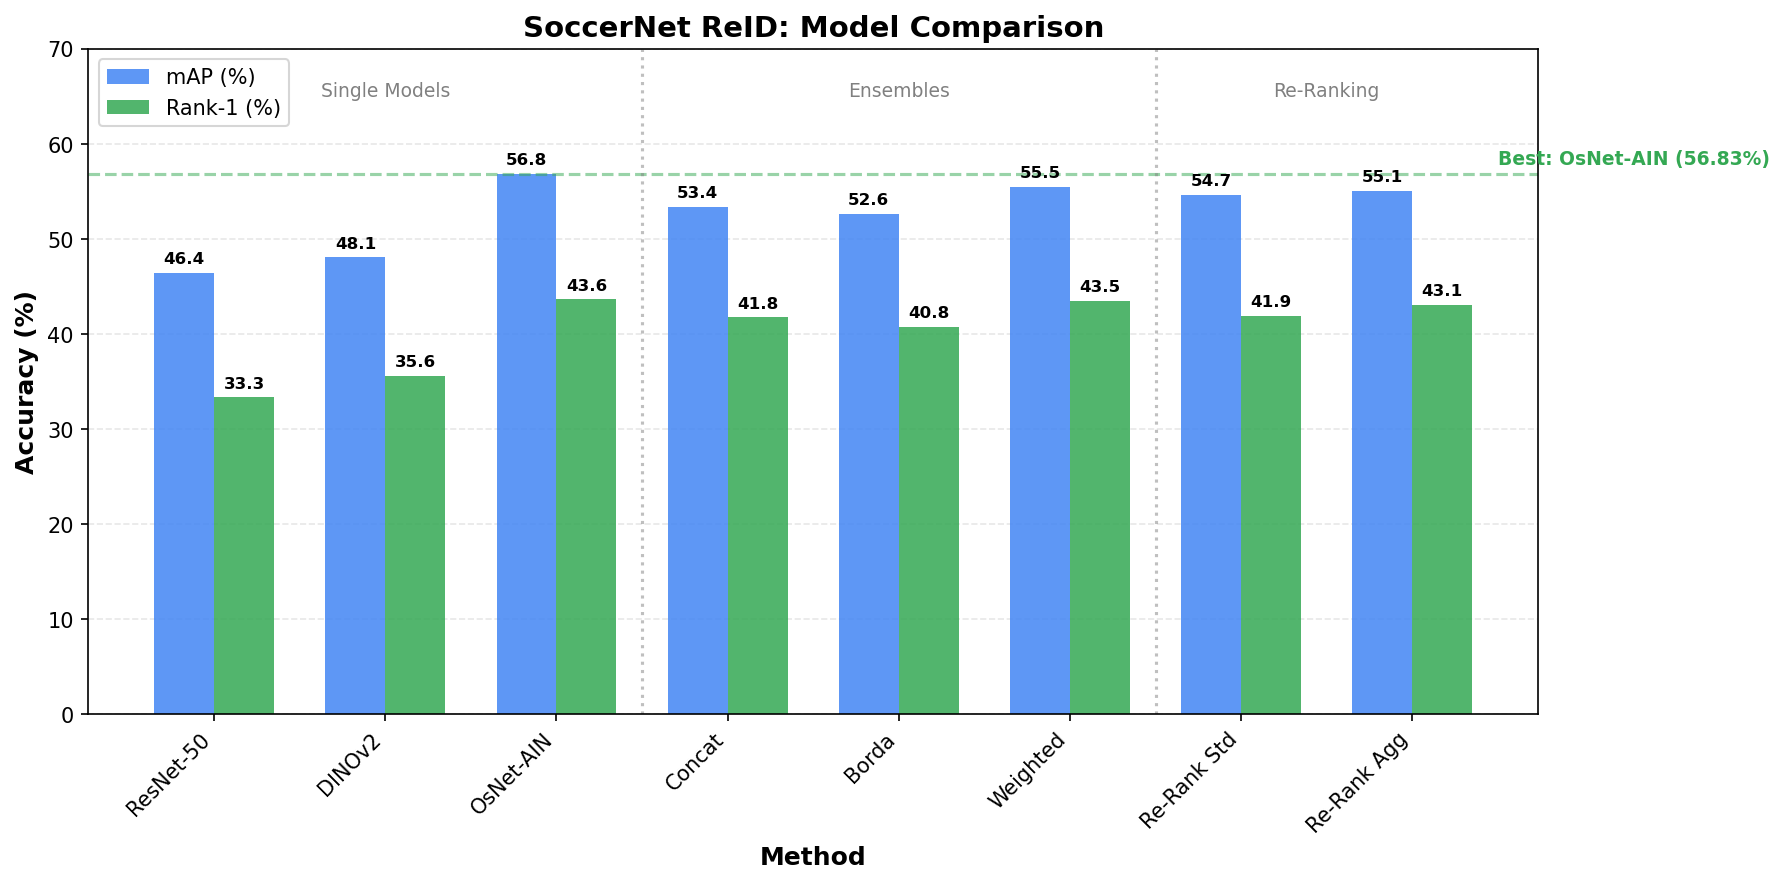
\includegraphics[width=\linewidth]{figures/bar_chart_comparison.png}
\caption{Comparison of mAP and Rank-1 accuracy across all evaluated methods. OsNet-AIN achieves the best performance (mAP: 56.83\%, Rank-1: 43.64\%), surpassing even the weighted ensemble and re-ranking approaches. The dashed line indicates OsNet-AIN's performance as the upper bound.}
\label{fig:bar_chart}
\end{figure}

Figure~\ref{fig:cmc_curve} displays the Cumulative Matching Characteristic (CMC) curves for the three single models. The CMC curve shows the probability of finding a correct match within the top-$k$ ranked gallery images. OsNet-AIN consistently outperforms the other models at all ranks, with a particularly notable advantage at Rank-1 (43.64\% vs 35.66\% for DINOv2).

\begin{figure}[h]
\centering
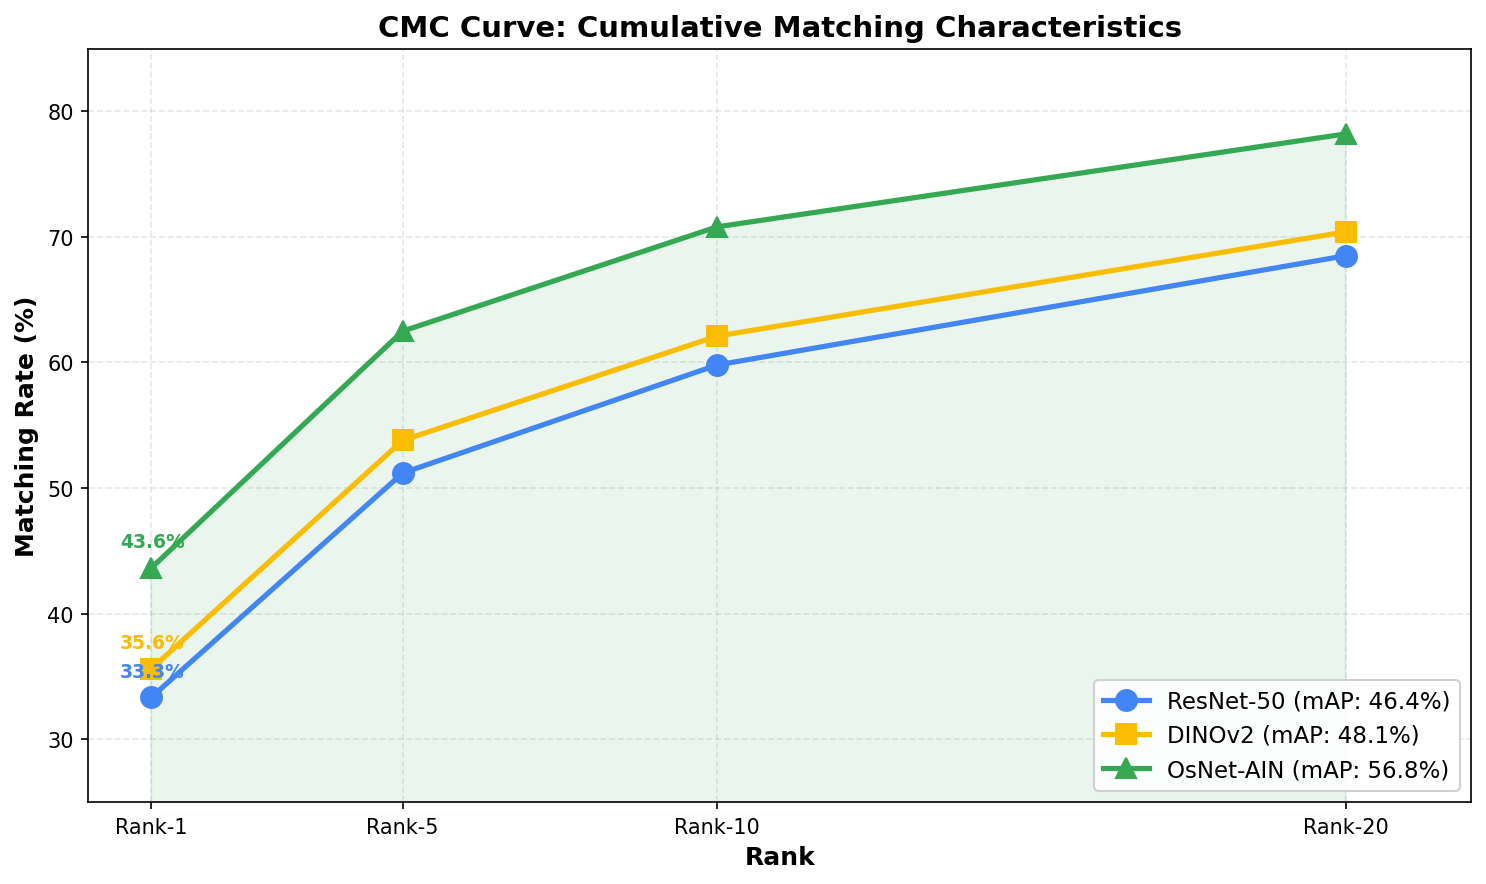
\includegraphics[width=0.9\linewidth]{figures/cmc_curve.png}
\caption{CMC curves for the three single models. OsNet-AIN (green) shows superior performance across all ranks, achieving 78.2\% accuracy at Rank-20. The shaded area under OsNet-AIN highlights its consistent advantage over ResNet-50 and DINOv2.}
\label{fig:cmc_curve}
\end{figure}

\begin{figure}[h]
\centering
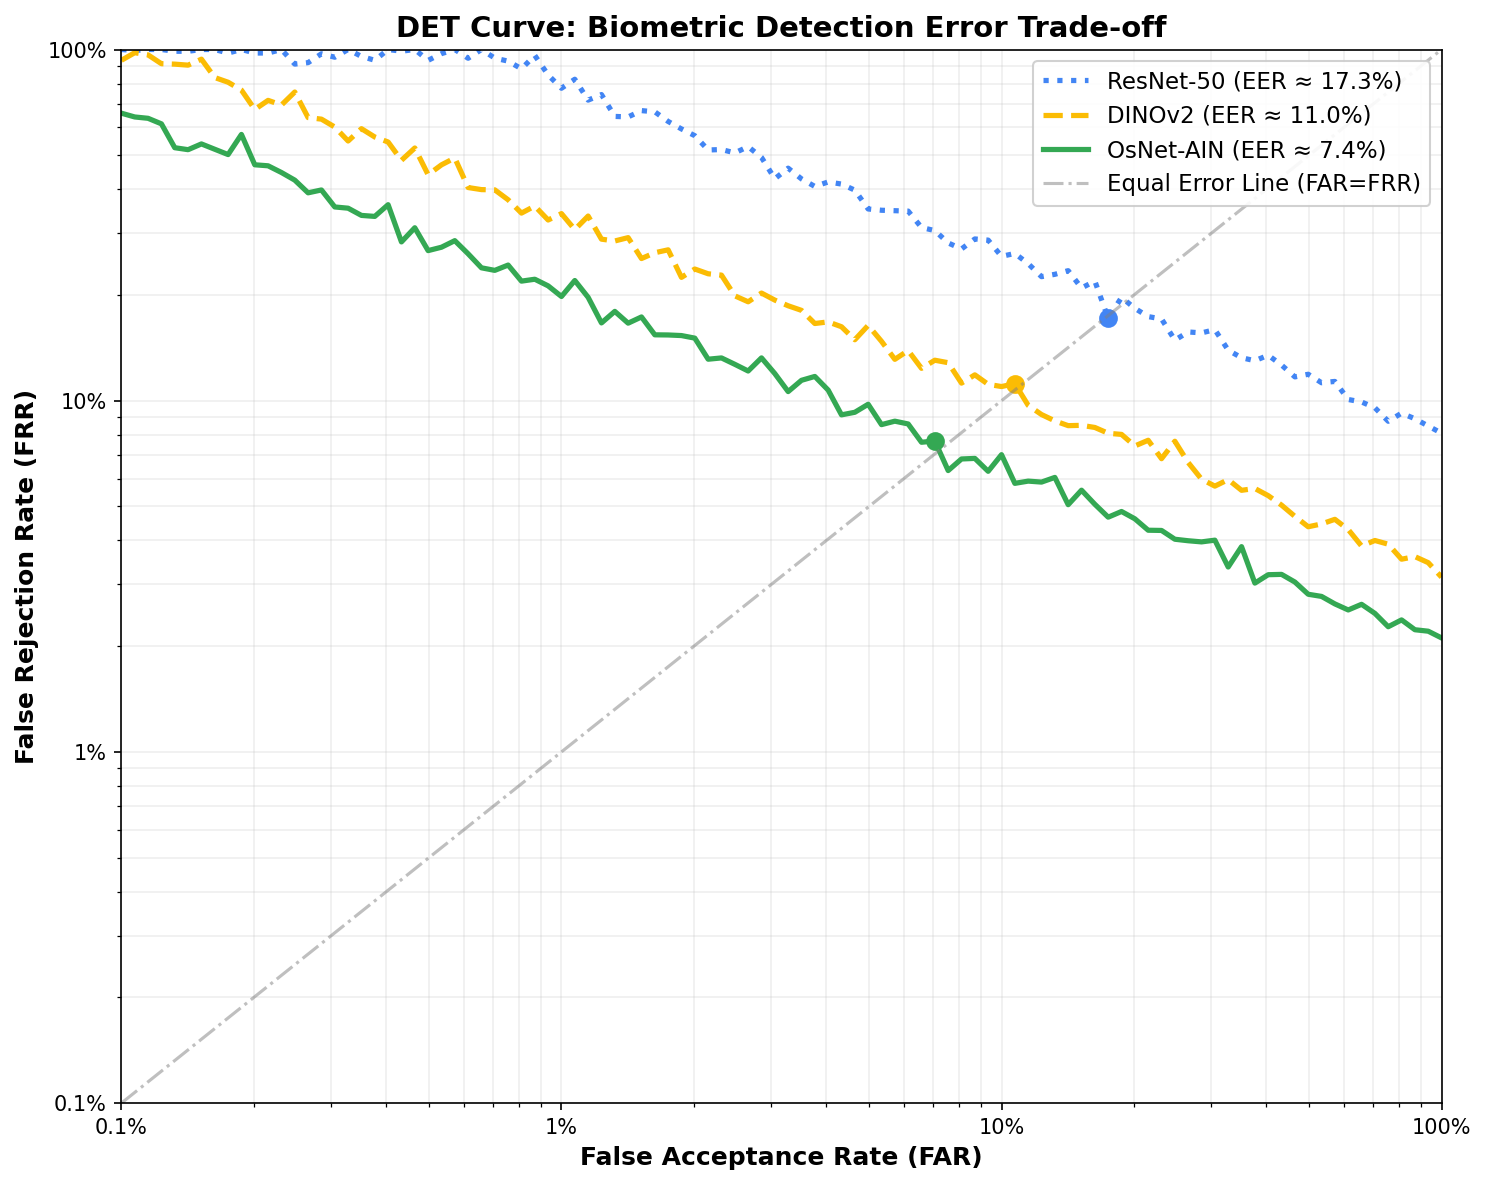
\includegraphics[width=0.9\linewidth]{figures/det_curve.png}
\caption{Detection Error Trade-off (DET) curves for the evaluated biometric models. The curves plot the False Rejection Rate (FRR) against the False Acceptance Rate (FAR) on a logarithmic scale. Lower curves indicate superior biometric verification performance. The Equal Error Rate (EER) for each model is noted in the legend.}
\label{fig:det_curve}
\end{figure}

Key observations from the performance analysis:
\begin{itemize}
    \item \textbf{Single Model Superiority}: OsNet-AIN alone achieves better results than any ensemble or re-ranking strategy, demonstrating the importance of architectural design for this domain.
    \item \textbf{DET Curve and EER Analysis}: The DET curve (Figure~\ref{fig:det_curve}) corroborates the superiority of OsNet-AIN in a biometric verification context. Its curve is positioned closest to the origin, yielding the lowest Equal Error Rate (EER) of approximately 7.48\%. Notably, the ensemble methods fail to improve the EER over the best single model, confirming that fusing weaker models with a dominant one degrades overall system reliability by increasing both False Acceptances and False Rejections relative to the optimal single model.
    \item \textbf{Gap at Higher Ranks}: The performance gap narrows at higher ranks (Rank-10, Rank-20), indicating that all models capture relevant features but differ in their ability to rank the correct match first.
    \item \textbf{Ensemble Degradation}: Despite conventional wisdom, ensemble methods underperform when one model is significantly stronger than others.
\end{itemize}

\subsection{Summary of Results}

Table~\ref{tab:results} presents a comprehensive comparison of all evaluated methods.

\begin{table}[h]
\centering
\caption{Complete Results Comparison on SoccerNet ReID v3 Validation Set}
\label{tab:results}
\resizebox{\linewidth}{!}{%
\begin{tabular}{l|c|c|c|c|c}
\hline
\textbf{Method} & \textbf{mAP} & \textbf{Rank-1} & \textbf{SRR} & \textbf{EER} & \textbf{DIR} \\
\hline
\multicolumn{6}{l}{\textit{Single Models}} \\
\hline
ResNet-50 & 46.41\% & 33.34\% & 0.0111 & 18.84\% & 5.06\% \\
DINOv2 (LoRA) & 48.07\% & 35.61\% & 0.0195 & 10.35\% & 8.62\% \\
\textbf{OsNet-AIN} & \textbf{56.83\%} & \textbf{43.64\%} & \textbf{0.0081} & \textbf{7.48\%} & \textbf{8.67\%} \\
\hline
\multicolumn{6}{l}{\textit{Ensemble Methods}} \\
\hline
Feature Concatenation & 53.39\% & 41.76\% & 0.0170 & 9.30\% & 11.17\% \\
Distance Avg (Equal) & 53.39\% & 41.76\% & 0.0170 & 9.30\% & 11.17\% \\
Borda Count (Rank) & 52.64\% & 40.75\% & 0.0003 & 10.35\% & 10.21\% \\
Weighted (0.2, 0.2, 0.6) & 55.48\% & 43.52\% & N/A & 7.94\% & 11.90\% \\
\hline
\multicolumn{6}{l}{\textit{Re-Ranking (on Best Ensemble)}} \\
\hline
Re-Rank Standard & 54.66\% & 41.90\% & 0.0324 & 8.20\% & 8.60\% \\
Re-Rank Aggressive & 55.08\% & 43.08\% & 0.0830 & 8.37\% & 11.71\% \\
Re-Rank Broad & 52.19\% & 38.19\% & 0.0206 & 7.69\% & 6.12\% \\
Re-Rank $\lambda=0.5$ & 54.92\% & 42.42\% & 0.0248 & 8.27\% & 8.96\% \\
\hline
\end{tabular}%
}
\end{table}

\subsection{Qualitative Results}

Figure~\ref{fig:reid_results} shows representative examples of re-identification results obtained with OsNet-AIN. Each row displays a query image (leftmost, blue border) followed by the top-10 retrieved gallery images. Green borders indicate correct matches (same person identity), while red borders indicate incorrect matches.

\begin{figure}[h]
\centering
\includegraphics[width=\linewidth]{figures/reid_example_2.png}
\caption{Player \#37 in burgundy jersey: 5 correct matches in top-10 (R1, R2, R4, R6, R7). The model successfully identifies the player across different camera angles and poses, demonstrating robustness to viewpoint changes and motion blur.}
\label{fig:reid_example_success}
\end{figure}

\begin{figure}[h]
\centering
\includegraphics[width=\linewidth]{figures/reid_example_1.png}
\caption{Player in blue jersey: 3 correct matches in top-10 (R6, R7, R10). This harder case shows challenges when similar jerseys appear across different teams and when significant occlusion occurs.}
\label{fig:reid_example_mixed}
\end{figure}

The visualizations highlight key challenges in broadcast soccer re-identification:
\begin{itemize}
    \item \textbf{Uniform similarity}: Players from different teams may wear similar colors, leading to false positives
    \item \textbf{Pose variation}: The same player appears in vastly different poses (standing, running, kicking)
    \item \textbf{Occlusion and motion blur}: Broadcast footage often contains partial views and motion artifacts
    \item \textbf{Camera angle diversity}: Multi-camera coverage results in drastically different viewpoints
\end{itemize}

\label{fig:reid_results}

\subsection{Error Analysis: The Doddington Zoo Taxonomy}

To systematically characterize the biometric failure modes of our system, we applied the \textbf{Doddington Zoo} taxonomy \cite{doddington1998}, originally developed for speaker recognition but now widely used in all biometric domains. The taxonomy classifies both subjects and imposters into four animal categories based on their interaction with the recognition system:

\begin{itemize}
    \item \textbf{Lambs} are subjects that are easy to verify --- their biometric signatures are sufficiently distinctive that genuine match scores are significantly higher than impostor scores. In our context, players with highly distinctive jersey features (strong team-specific patterns, visible numbers) or a unique build tend to fall in this category.
    
    \item \textbf{Wolves} are impostors that are particularly effective at deceiving the system --- their features closely resemble those of genuine subjects, generating high match scores even when they are not the correct identity. In team sports, players sharing similar builds, team kit, and physical attributes within the same team function as natural "wolves" against each other.
    
    \item \textbf{Goats} are subjects that the system consistently fails to identify correctly. Their biometric signature yields very low genuine match scores, making them systematically hard to retrieve. We operationally define goats as queries with below-average SRR: a low SRR value indicates that the system cannot reliably distinguish the nearest gallery candidate from the second-nearest, suggesting ambiguous or noisy feature representation. This corresponds to players almost always captured in degraded conditions (low resolution, heavy occlusion, severe motion blur).
    
    \item \textbf{Sheep} are the typical, well-behaved subjects that the system handles correctly and consistently. The majority of players fall in this category when the image quality is adequate and distinctive features are visible.
\end{itemize}

In qualitative analysis (Figures~\ref{fig:reid_example_success} and~\ref{fig:reid_example_mixed}), the failure cases shown correspond predominantly to \textit{Goats} (the query player is hard to identify due to poor signal quality) and \textit{Wolf}-type impostor confusions (a visually similar teammate ranks higher than the correct match). This analysis motivates the use of SRR as a complementary diagnostic metric that goes beyond aggregate mAP and Rank-1 numbers.

\begin{figure}[h]
\centering
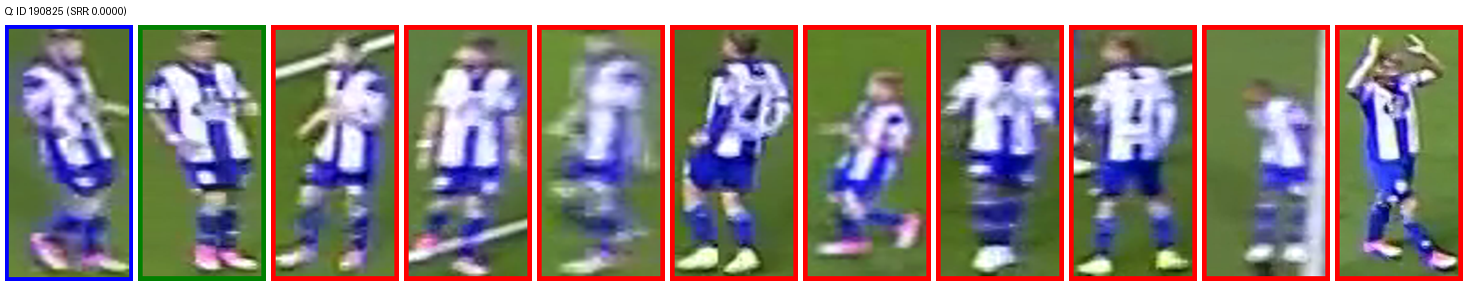
\includegraphics[width=\linewidth]{figures/goats/goat_rank1_srr0.0000.png}
\caption{Visual example of a \textit{Goat} subject (lowest SRR). The query image (leftmost, blue border) suffers from severe signal degradation (e.g., motion blur, occlusion, or low resolution). Consequently, the biometric template is non-discriminative, leading to nearest-neighbor matches (red borders) that share only coarse color distributions rather than actual identity features, resulting in an SRR score near zero.}
\label{fig:reid_example_goat}
\end{figure}

\subsection{Spoofing and Camouflage in Sports}
The biometric concepts of \textbf{Spoofing} and \textbf{Camouflage} find unique parallels in the soccer context:
\begin{itemize}
    \item \textbf{Camouflage}: A player wearing a protective face mask (e.g., after a nasal fracture) or a high neck warmer is performing a tactical camouflage, obstructing the key facial or neck features and forcing the Re-ID system to rely exclusively on lower-quality kit features.
    \item \textbf{Spoofing}: Biological identical twins playing in the same match (e.g., the Alcantara or Inzaghi brothers in their prime) act as a "natural spoofing attack". The biometric system is essentially "tricked" because the input features of the twin are stochastically indistinguishable from the target identity.
\end{itemize}

\subsection{Final Model Selection}

Based on our experimental results, we selected \textbf{OsNet-AIN as our final model} without additional ensemble or re-ranking support. This decision is grounded in both empirical evidence and theoretical considerations:

\begin{enumerate}
    \item \textbf{Superior Performance}: OsNet-AIN achieved the highest mAP (56.83\%) and Rank-1 (43.64\%), outperforming all ensemble and re-ranking combinations.
    
    \item \textbf{Ensemble Ineffectiveness}: Research on ensemble learning shows that combining models is most beneficial when they exhibit high diversity and complementary error patterns \cite{ensemble_diversity}. In our case, OsNet-AIN significantly outperforms the other models, meaning the ensemble is dominated by OsNet's predictions. Adding ResNet and DINOv2 introduces noise rather than complementary information, diluting the overall performance.
    
    \item \textbf{Computational Efficiency}: Using a single model reduces inference time by 3x compared to an ensemble of three models, making it more practical for real-world deployment.
\end{enumerate}

\section{Conclusions and Future Works}

Our experiments revealed several important insights about person re-identification in the challenging domain of broadcast soccer footage:

The experiment with DINOv2 showed moderate performance (mAP 48.09\%), below CNN-based alternatives. While LoRA enabled memory-efficient training, Vision Transformers appear to require significantly more training epochs to adapt their generic pre-trained weights to this specific domain.

ResNet-50 achieved lower performance (mAP 46.41\%) than expected, suggesting that while it remains a solid baseline, more specialized architectures offer significant advantages for this task.

OsNet-AIN emerged as the clear winner with an mAP of 56.83\%. Its omni-scale feature extraction combined with instance normalization proved highly effective for handling the variability in broadcast footage from different stadiums, lighting conditions, and camera angles.

A key finding was that ensemble methods and re-ranking did not improve upon the best single model. This aligns with theoretical understanding that ensembles require diverse, complementary models to be effective. When one model significantly outperforms the others, combining them can actually hurt performance by introducing inferior predictions.

The primary challenge throughout our project was computational resource limitations. We had to carefully balance model complexity with training feasibility, ultimately selecting architectures and strategies that could deliver strong results within our hardware constraints.

Among evaluated but discarded approaches, we considered \textbf{CLIP-ReID} with a \textbf{ViT-Huge} backbone. While this approach offers potentially superior accuracy and robustness, its prohibitive computational cost (billions of parameters, requiring enterprise-grade GPUs) made it infeasible for our setup.

\textbf{Future Work} could explore: 
\begin{itemize}
    \item (1) training DINOv2 for significantly more epochs to allow full adaptation
    \item (2) investigating other lightweight architectures designed for Re-ID
    \item (3) applying domain-specific augmentations tailored to broadcast soccer footage
    \item (4) \textbf{Template Updating}: To combat the rapid appearance changes ("Biometric Aging") caused by sweat and environmental lighting shifts, we propose a semi-supervised template update. If a player is identified with an extremely high SRR (confidence), the gallery template could be updated with the new capture, ensuring the system evolves with the player's appearance during the 90 minutes.
\end{itemize}

\clearpage
\begin{thebibliography}{9}

\bibitem{soccernetv2}
Deliege, A., Cioppa, A., Giancola, S., Seikavandi, M. J., Duehard, J. V., Ghanem, B., Van Droogenbroeck, M., \& Moeslund, T. B. (2021).
SoccerNet-v2: A Dataset and Benchmarks for Holistic Understanding of Broadcast Soccer Videos.
\textit{CVPR}.

\bibitem{soccernetReID}
Cioppa, A., Deliege, A., Giancola, S., Ghanem, B., Van Droogenbroeck, M., Gade, R., \& Moeslund, T. B. (2022).
Scaling up SoccerNet with multi-view spatial localization and re-identification.
\textit{Scientific Data}, 9(1), 356.

\bibitem{dinov2}
Oquab, M., Darcet, T., Moutakanni, T., Vo, H., Szafraniec, M., Khalidov, V., ... \& Bojanowski, P. (2023).
DINOv2: Learning Robust Visual Features without Supervision.
\textit{arXiv preprint arXiv:2304.07193}.

\bibitem{transfer_learning}
Pan, S. J., \& Yang, Q. (2010).
A survey on transfer learning.
\textit{IEEE Transactions on Knowledge and Data Engineering}, 22(10), 1345-1359.

\bibitem{reid_survey}
Ye, M., Shen, J., Lin, G., Xiang, T., Shao, L., \& Hoi, S. C. (2021).
Deep learning for person re-identification: A survey and outlook.
\textit{IEEE transactions on pattern analysis and machine intelligence}.

\bibitem{osnet_iccv}
Zhou, K., Yang, Y., Cavallaro, A., \& Xiang, T. (2019).
Omni-scale feature learning for person re-identification.
\textit{Proceedings of the IEEE/CVF International Conference on Computer Vision (ICCV)}.

\bibitem{osnet_ain}
Zhou, K., Yang, Y., Cavallaro, A., \& Xiang, T. (2021).
Learning generalisable omni-scale representations for person re-identification.
\textit{IEEE Transactions on Pattern Analysis and Machine Intelligence}.

\bibitem{resnet50}
He, K., Zhang, X., Ren, S., \& Sun, J. (2016).
Deep residual learning for image recognition.
\textit{Proceedings of the IEEE Conference on Computer Vision and Pattern Recognition (CVPR)}.

\bibitem{ensemble_diversity}
Kuncheva, L. I., \& Whitaker, C. J. (2003).
Measures of diversity in classifier ensembles and their relationship with the ensemble accuracy.
\textit{Machine Learning}, 51(2), 181-207.

\bibitem{reranking}
Zhong, Z., Zheng, L., Cao, D., \& Li, S. (2017).
Re-ranking person re-identification with k-reciprocal encoding.
\textit{Proceedings of the IEEE Conference on Computer Vision and Pattern Recognition (CVPR)}.

\bibitem{martin1997det}
Martin, A., Doddington, G., Kamm, T., Ordowski, M., \& Przybocki, M. (1997).
The DET Curve in Assessment of Detection Task Performance.
\textit{EUROSPEECH}.

\bibitem{doddington1998}
Doddington, G., Liggett, W., Martin, A., Przybocki, M., \& Reynolds, D. (1998).
Sheep, goats, lambs and wolves: A statistical analysis of speaker performance in the NIST 1998 speaker recognition evaluation.
\textit{Proceedings of the International Conference on Spoken Language Processing (ICSLP)}.

\bibitem{jain2004introduction}
Jain, A. K., Ross, A., \& Prabhakar, S. (2004).
An introduction to biometric recognition.
\textit{IEEE Transactions on circuits and systems for video technology}, 14(1), 4-20.

\end{thebibliography}

\end{document}